\documentclass{article}
\usepackage[utf8x]{inputenc}
\usepackage[T1]{fontenc}
\usepackage[french]{babel}
\usepackage{graphicx}
\usepackage{vmargin}
\usepackage{moreverb}
\usepackage{tikz}
\usepackage{algpseudocode}
\usepackage{algorithm}
%\usepackage{algorithmicx}
\setmarginsrb{2cm}{2cm}{2cm}{2cm}{0cm}{0cm}{0cm}{0cm}

\frenchbsetup{StandardLists=true}


\title{Logique: prise de note groupe 23}
\author{Bellenger Jordan \and Schmitz Loic }
\date{\today}

\begin{document}

\maketitle
\section{Chapitre 13: Structure du Web}


\subsection{Mémoire associative-Hypertexte}

$
\left. \text{\parbox{0.5\linewidth}{
\begin{itemize}
\item Graphe de citations : précurseur 
\item Renvois dans une encyclopédie (Wikipédia)
\end{itemize}
}}\right\}
$ Réseaux d'informations




\begin{figure}[!h]
\centering
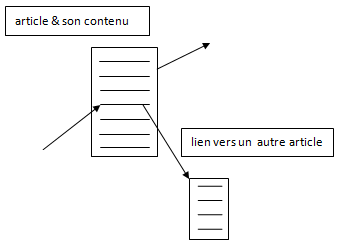
\includegraphics{images/23_image1.png}
\caption{Hypertexte -liens vers des articles}
\label{fig:cfc}
\end{figure}

\textbf{Problème de cohérence}

\begin{itemize}
\item \underline{Web}: Cohérence \textit{"a posteriori"} \\
                       On va avoir besoin d'utiliser un outil afin d'imposer                         une structure : un moteur de recherche. 
      
\item \underline{Wikipedia}: Cohérence \textit{"a priori"} \\
                             Une structure existe déjà, définie par les                                    organisateurs. C'est déjà organisé.
\end{itemize}

Le succès du Web réside dans la possibilité de trouver une structure à ce dernier. Notamment grâce au Pagerank. Altavista, Google, Lycos, ... proposent tous leur version de moteur de recherche. Au fil du temps, Google a su s'imposer largement grâce à la qualité de son outil.

\subsection{Le Web est un graphe orienté}
\begin{itemize}
\item \underline{Chemin dans un graphe orienté}: A ---> B\\
Séquene de noeuds qui commence avec A et termine avec B et où chaque paire consécutive correspond à un lien orienté.

\item \underline{Connectivité}: \\
Un graphe orienté est connexe s'il existe un chemin orienté entre chaque paire de noeuds.
\end{itemize}

\subsection{Composant fortement connexe (CFC) \textit{- Strongly Connected Component (SCC)} }
\\
Dans un graphe orienté :
\begin{itemize}
    \item Ensemble de noeuds tel qu'il existe un chemin orienté entre                   chaque paire.
    \item L'ensemble ne fait pas partie d'un plus grand environnement qui               à la même propriété. 
\end{itemize}

Les CFCs forment un genre de \textit{"super noeud"}. Pour la connectivité, il n'y a que les CFCs qui comptent.
\\


Il faut transformer le graphe en un graphe réduit : le CFC devient 1 seul "super gros" noeud. Pour trouver un chemin dans le graphe original, il suffit de trouver un chemin dans le graphe réduit. Ref : Figure 13.6
\\

\begin{figure}[!h]
\centering
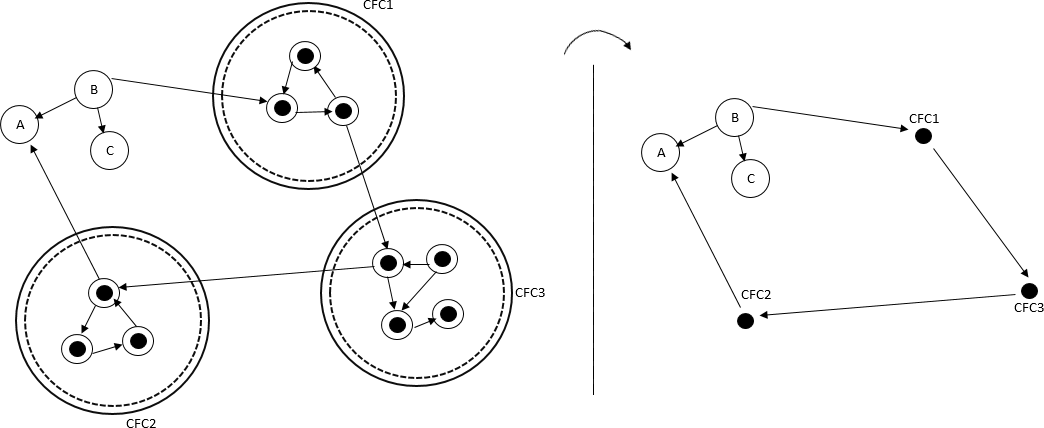
\includegraphics[width=500px]{images/23_schema2.png}
\caption{Exemple de transformation du graphe}
\label{fig:cfc}
\end{figure}

\subsection{Noeud de papillon \textit{ $\approx$ années 2000}}
Ref: Figure 13.7


\subsection{L'émergence du Web 2.0  \textit{$\ge$ années 2000}}
L'émergence du Web 2.0 se déroule entre 2000 et 2010. Il s'agit en fait d'un changement d'attitude général conduisant à une structuration de la toile basé sur 3 grands principes principalement. \\
\begin{enumerate}
    \item Création \underline{collaborative} de contenu plutôt que des pages personnelles.
    
    \item \underline{Services}: Transfert des données personnelles vers les services. Au lieu de publier du contenu personnel (images, vidéos, ...) les gens se tournent vers des services comme YouTube par exemple ou Flickr, ...
    \item \underline{Personnes} au lieu des documents (liens faisant référence à des personnes.
\end{enumerate} 

\vspace * {0.3cm}
\begin{minipage}{15cm}
\textbf{Technologies utilisées:}
    \begin{itemize}
        \item Blogs 
        \item Deep Web : création de page à la demande 
        \item Cloud : grandes ressources élastiques (change de taille                      selon les besoins) 
    \end{itemize}
\end{minipage}

\vspace{0.5cm}       

\newpage

\hline 
\vspace * {0.5cm}
    \fbox{\textbf{Un petit bout d'histoire}}\\
    
    \underline{Quelques précurseurs} :
    
    \begin{itemize}
        \item \underline{1945 - Vannevar Bush} : Conseiller du président des États-Unis, Roosevelt\\ 
        Il a écrit un article intitulé "As We May Think" dans lequel il explique son appareil électronique relié à une bibliothèque et capable d'afficher des livres et de projeter des films appelé "Memex".
        \item \underline{1934 - Paul Otlet} : Documentaliste\\ 
        C'est lui qui a eu la première intuition de l'internet, il avait imaginé, à l'époque, à un système où l'on pourrait faire des recherches et où on pourrait consulter le résultat de ces recherches sur un écran. Ce qui fait fortement penser à l'internet d'aujourd'hui. Il a aussi inventé les microfiches.
        \item \underline{1990 - Tim Berners-Lee et  Robert Cailliau - CERN} : Inventeur du World Wide Web\\
        Ils se sont inspirés des ecrits de Vannevar Bush pour inventer le WWW
    \end{itemize}
    
\vspace * {0.5cm}   
\hline 


\section{Chapitre 14: Recherche dans le Web}
Comment trouver une information ?\\

\underline{1960}:Concept de mot-clé => Limitations fortes

\begin{itemize}
    \item Limitations dûes au concept de mots 
        \begin{itemize}
            \item Synonymie : plusieurs mots pour le même concept.
            \item Polynomie : un mot pour plusieurs concepts.\\
            \underline{Exemple}: Pour le mot "Cornell": il y a 3 concepts
                 \begin{itemize}
                    \item Université de Cornell
                    \item Eric Cornell (Prix Nobel 2001) 
                    \item Equipe de Hockey
                 \end{itemize}

        \end{itemize}
    \item Limitations dûes à l'abondance d'informations. \\
    $\left. \text{\parbox{0.5\linewidth}{
        \begin{itemize}
            \item \underline{Avant}: Les informations sur le web étaient rares. 
            \item \underline{Maintenant}: Il y a beaucoup trop d'informations.
        \end{itemize}
        }} \right \}$ Plus grand problème du web
\end{itemize}
    
$\Rightarrow$ Pour solutionner ce problème d'abondance, l'utilisation de la structure du réseau est nécessaire pour trouver les informations les plus fiables.


\end{document}



